% ============================================================================
% PAPER MODIFICATIONS FOR GAN HPO EXPERIMENT
% ============================================================================
% This file contains all text modifications needed to add the GAN HPO
% experiment to the BIF paper. Each section is clearly labeled with the
% paragraph/location that needs to be modified.
%
% Figure components (you assemble the composite figure):
%   Panel A: figures/dcgan_combined2_v2.png  (DCGAN architecture + surrogate landscape)
%   Panel B: figures/v3_fair_main_ro.png     (Main RO)
%   Panel C: figures/v3_fair_main_r2.png     (Main Parent R2 + Child R2)
%   Panel D: figures/dcgan_combined2_v2_specnorm.png  (SpectralNorm disc landscape)
%   Panel E: figures/v3_fair_modularity_ro.png  (Modularity RO)
%   Panel F: figures/v3_fair_modularity_r2.png  (Modularity Parent R2 + Child R2)
%   Panel G: results table (included below as LaTeX)
% ============================================================================


% ============================================================================
% MODIFICATION 1: Section 4 "Datasets" — ADD new bullet point
% Location: After the Neurostimulation bullet point (line ~164 in main_paper.md)
% Add the following as a 4th bullet:
% ============================================================================

\paragraph{Datasets --- add 4th bullet after Neurostimulation:}

\begin{itemize}
\item GAN Hyperparameter Optimization: A tabular surrogate built from 2{,}401
DCGAN training runs on Fashion-MNIST, spanning a $7^4$ grid over four
hyperparameters split into two functional groups: generator
(learning rate, weight decay) and discriminator (learning rate, dropout).
Each configuration was trained to convergence and scored by FID.
A second surrogate replaces the standard discriminator with a
Spectral-Norm variant, sharing the generator architecture.
This pair of surrogates enables testing BIF's modularity:
the generator child trained on the standard task can be transferred
to the Spectral-Norm task without retraining, since only the
discriminator sub-problem changes.
\end{itemize}


% ============================================================================
% MODIFICATION 2: Section 4 "Datasets" — UPDATE opening sentence
% Location: First sentence of Datasets paragraph (line ~160)
% Change "three benchmarks" to "four benchmarks"
% ============================================================================

\paragraph{Datasets --- update opening sentence:}

% OLD: "We evaluate BIF on three benchmarks designed to test hierarchical
%       transfer and scalability."
% NEW:
We evaluate BIF on four benchmarks designed to test hierarchical
transfer and scalability.


% ============================================================================
% MODIFICATION 3: Section 4 "Implementation Details" — ADD GAN-specific note
% Location: End of Implementation Details paragraph (line ~170)
% Append the following sentence:
% ============================================================================

\paragraph{Implementation Details --- append at end of paragraph:}

For the GAN surrogate, we use $\kappa\!=\!20$, $\gamma\!=\!4$,
$\nu\!=\!1.5$, with a log-normal lengthscale prior centered at 1.0.
All methods share the same 20-query parent budget;
BIF and Laferri\`ere each use 3 initialization queries
(counted in the budget). Results report mean and standard error
across 30 randomly initialized trials.


% ============================================================================
% MODIFICATION 4: Section 4 "Implementation Details" — UPDATE trial count
% Location: Last sentence "Results report the mean and standard error
%           across 10 randomly initialized trials."
% ============================================================================

\paragraph{Implementation Details --- update trial count:}

% OLD: "Results report the mean and standard error across 10 randomly
%       initialized trials."
% NEW:
Results report the mean and standard error across 10 randomly
initialized trials (30 for the GAN surrogate).


% ============================================================================
% MODIFICATION 5: Section 5 "Results" — ADD new subsection after
%                 "Real-World Application: Neurostimulation"
% Location: After the Neurostimulation results paragraph, before
%           "Modularity and Subtask Transfer" (between lines ~234 and ~236)
% ============================================================================

\paragraph{Results --- insert new subsection ``GAN Hyperparameter Optimization'':}

\textbf{GAN Hyperparameter Optimization.}
We evaluate BIF on a tabular DCGAN surrogate (Section~4),
where the generator and discriminator form natural child sub-problems
within a joint 4D parent space.
As summarized in Table~1 and Figure~4(a--c), BIF matches vanilla
GPBO in Relative Optimum ($96.1 \pm 0.4$ vs.\ $96.0 \pm 0.4$) while
achieving the highest parent $R^2$ ($11.4\%$) and child $R^2$ ($27.7\%$)
among all methods.
Laferri\`ere lags in both RO ($94.7 \pm 0.6$) and child $R^2$ ($23.1\%$),
confirming that frozen children limit the hierarchy's ability to
refine sub-task representations.
Although parent $R^2$ remains modest across all methods due to the
difficulty of modelling 2{,}401 points from only 20 queries,
BIF's child $R^2$ rises steadily (Fig.~4c),
driven by the response contribution system (Section~3).
The Laferri\`ere children, by contrast, plateau immediately after
initialization, as no downward signal reaches them.


% ============================================================================
% MODIFICATION 6: Section 5 "Modularity and Subtask Transfer" —
%                 REPLACE or EXTEND with GAN modularity results
% Location: The existing "Modularity and Subtask Transfer" paragraph
%           (lines ~236--240). Keep the existing text and append a new
%           paragraph about GAN modularity after it.
% ============================================================================

\paragraph{Modularity and Subtask Transfer --- append new paragraph:}

We further validate modularity on the GAN surrogate, where the generator
architecture is shared between the standard and Spectral-Norm
discriminator tasks.
As shown in Figure~4(d--f) and Table~1, BIF hot-start transfers
the pre-trained generator child and continues to refine both children
on the new task, reaching $95.3 \pm 0.5$ RO and $45.6\%$ child $R^2$.
Laferri\`ere hot-start carries the same generator child but freezes it,
achieving only $93.3 \pm 0.5$ RO and $23.2\%$ child $R^2$ ---
nearly half of BIF's child accuracy.
Vanilla GPBO, starting from scratch without any transferred knowledge,
reaches $93.5 \pm 0.7$ RO.


% ============================================================================
% MODIFICATION 7: Section 6 "Conclusion" — UPDATE to mention GAN experiment
% Location: Second paragraph of Conclusion (line ~246), which lists the
%           empirical evaluations.
% ============================================================================

\paragraph{Conclusion --- update empirical summary sentence:}

% OLD: "Empirical evaluations on 2D and 3D synthetic benchmarks, as well
%       as a real-world neurostimulation task, demonstrate that BIF
%       significantly improves sample efficiency..."
% NEW:
Empirical evaluations on synthetic benchmarks, a real-world
neurostimulation task, and a realistic GAN hyperparameter optimization surrogate
demonstrate that BIF significantly improves sample efficiency,
with higher AUC across the board, and overall optimization performance.


% ============================================================================
% MODIFICATION 8: Table 1 — ADD GAN rows
% Location: Table 1 (lines ~191--201). Add two new row groups at the bottom.
% ============================================================================

\paragraph{Table 1 --- add GAN rows:}

% Add these rows to Table 1, after the Neural Stimulation rows:

\begin{table}[h]
\caption{Summary of performance metrics.
GAN results use 20 queries and 30 seeds;
other datasets use 100 queries and 10 seeds.
Vanilla GPBO has no child $R^2$ (non-hierarchical).
Performance metrics are described in Section~4.}
\label{tab:results}
\centering
\small
\begin{tabular}{llcccc}
\toprule
Dataset & Model & Relative Optimum & Parent $R^2$ & Child $R^2$ & Global AUC \\
\midrule
% ... existing rows for Synthetic 2D, 3D, Neural Stimulation ...
\midrule
GAN HPO         & Vanilla GPBO   & $96.0 \pm 0.4$ & $9.7 \pm 1.0$  & --              & $95.1 \pm 0.4$ \\
                & Laferri\`ere   & $94.7 \pm 0.6$ & $6.8 \pm 1.1$  & $23.1 \pm 2.4$  & $92.0 \pm 0.4$ \\
                & BIF            & $96.1 \pm 0.4$ & $11.4 \pm 1.3$ & $27.7 \pm 2.9$  & $94.9 \pm 0.4$ \\
\midrule
GAN HPO         & Vanilla GPBO   & $93.5 \pm 0.7$ & $43.7 \pm 1.0$ & --              & $91.9 \pm 0.8$ \\
(Modularity)    & Laferri\`ere   & $93.3 \pm 0.5$ & $48.8 \pm 1.0$ & $23.2 \pm 2.4$  & $88.5 \pm 0.7$ \\
                & BIF            & $95.3 \pm 0.5$ & $48.5 \pm 1.2$ & $45.6 \pm 2.6$  & $91.0 \pm 0.5$ \\
\bottomrule
\end{tabular}
\end{table}


% ============================================================================
% MODIFICATION 9: Figure 4 — NEW composite figure
% Location: Near the GAN results text (after Figure 3 / before Modularity,
%           or as a float near the new GAN subsection)
% ============================================================================

\paragraph{Figure 4 --- new composite figure:}

\begin{figure*}[t]
\centering
% You will assemble this manually. Panels:
% (a) dcgan_combined2_v2.png         — DCGAN architecture + standard surrogate
% (b) v3_fair_main_ro.png            — Main experiment: RO
% (c) v3_fair_main_r2.png            — Main experiment: Parent R2 + Child R2
% (d) dcgan_combined2_v2_specnorm.png — SpectralNorm discriminator landscape
% (e) v3_fair_modularity_ro.png      — Modularity: RO
% (f) v3_fair_modularity_r2.png      — Modularity: Parent R2 + Child R2
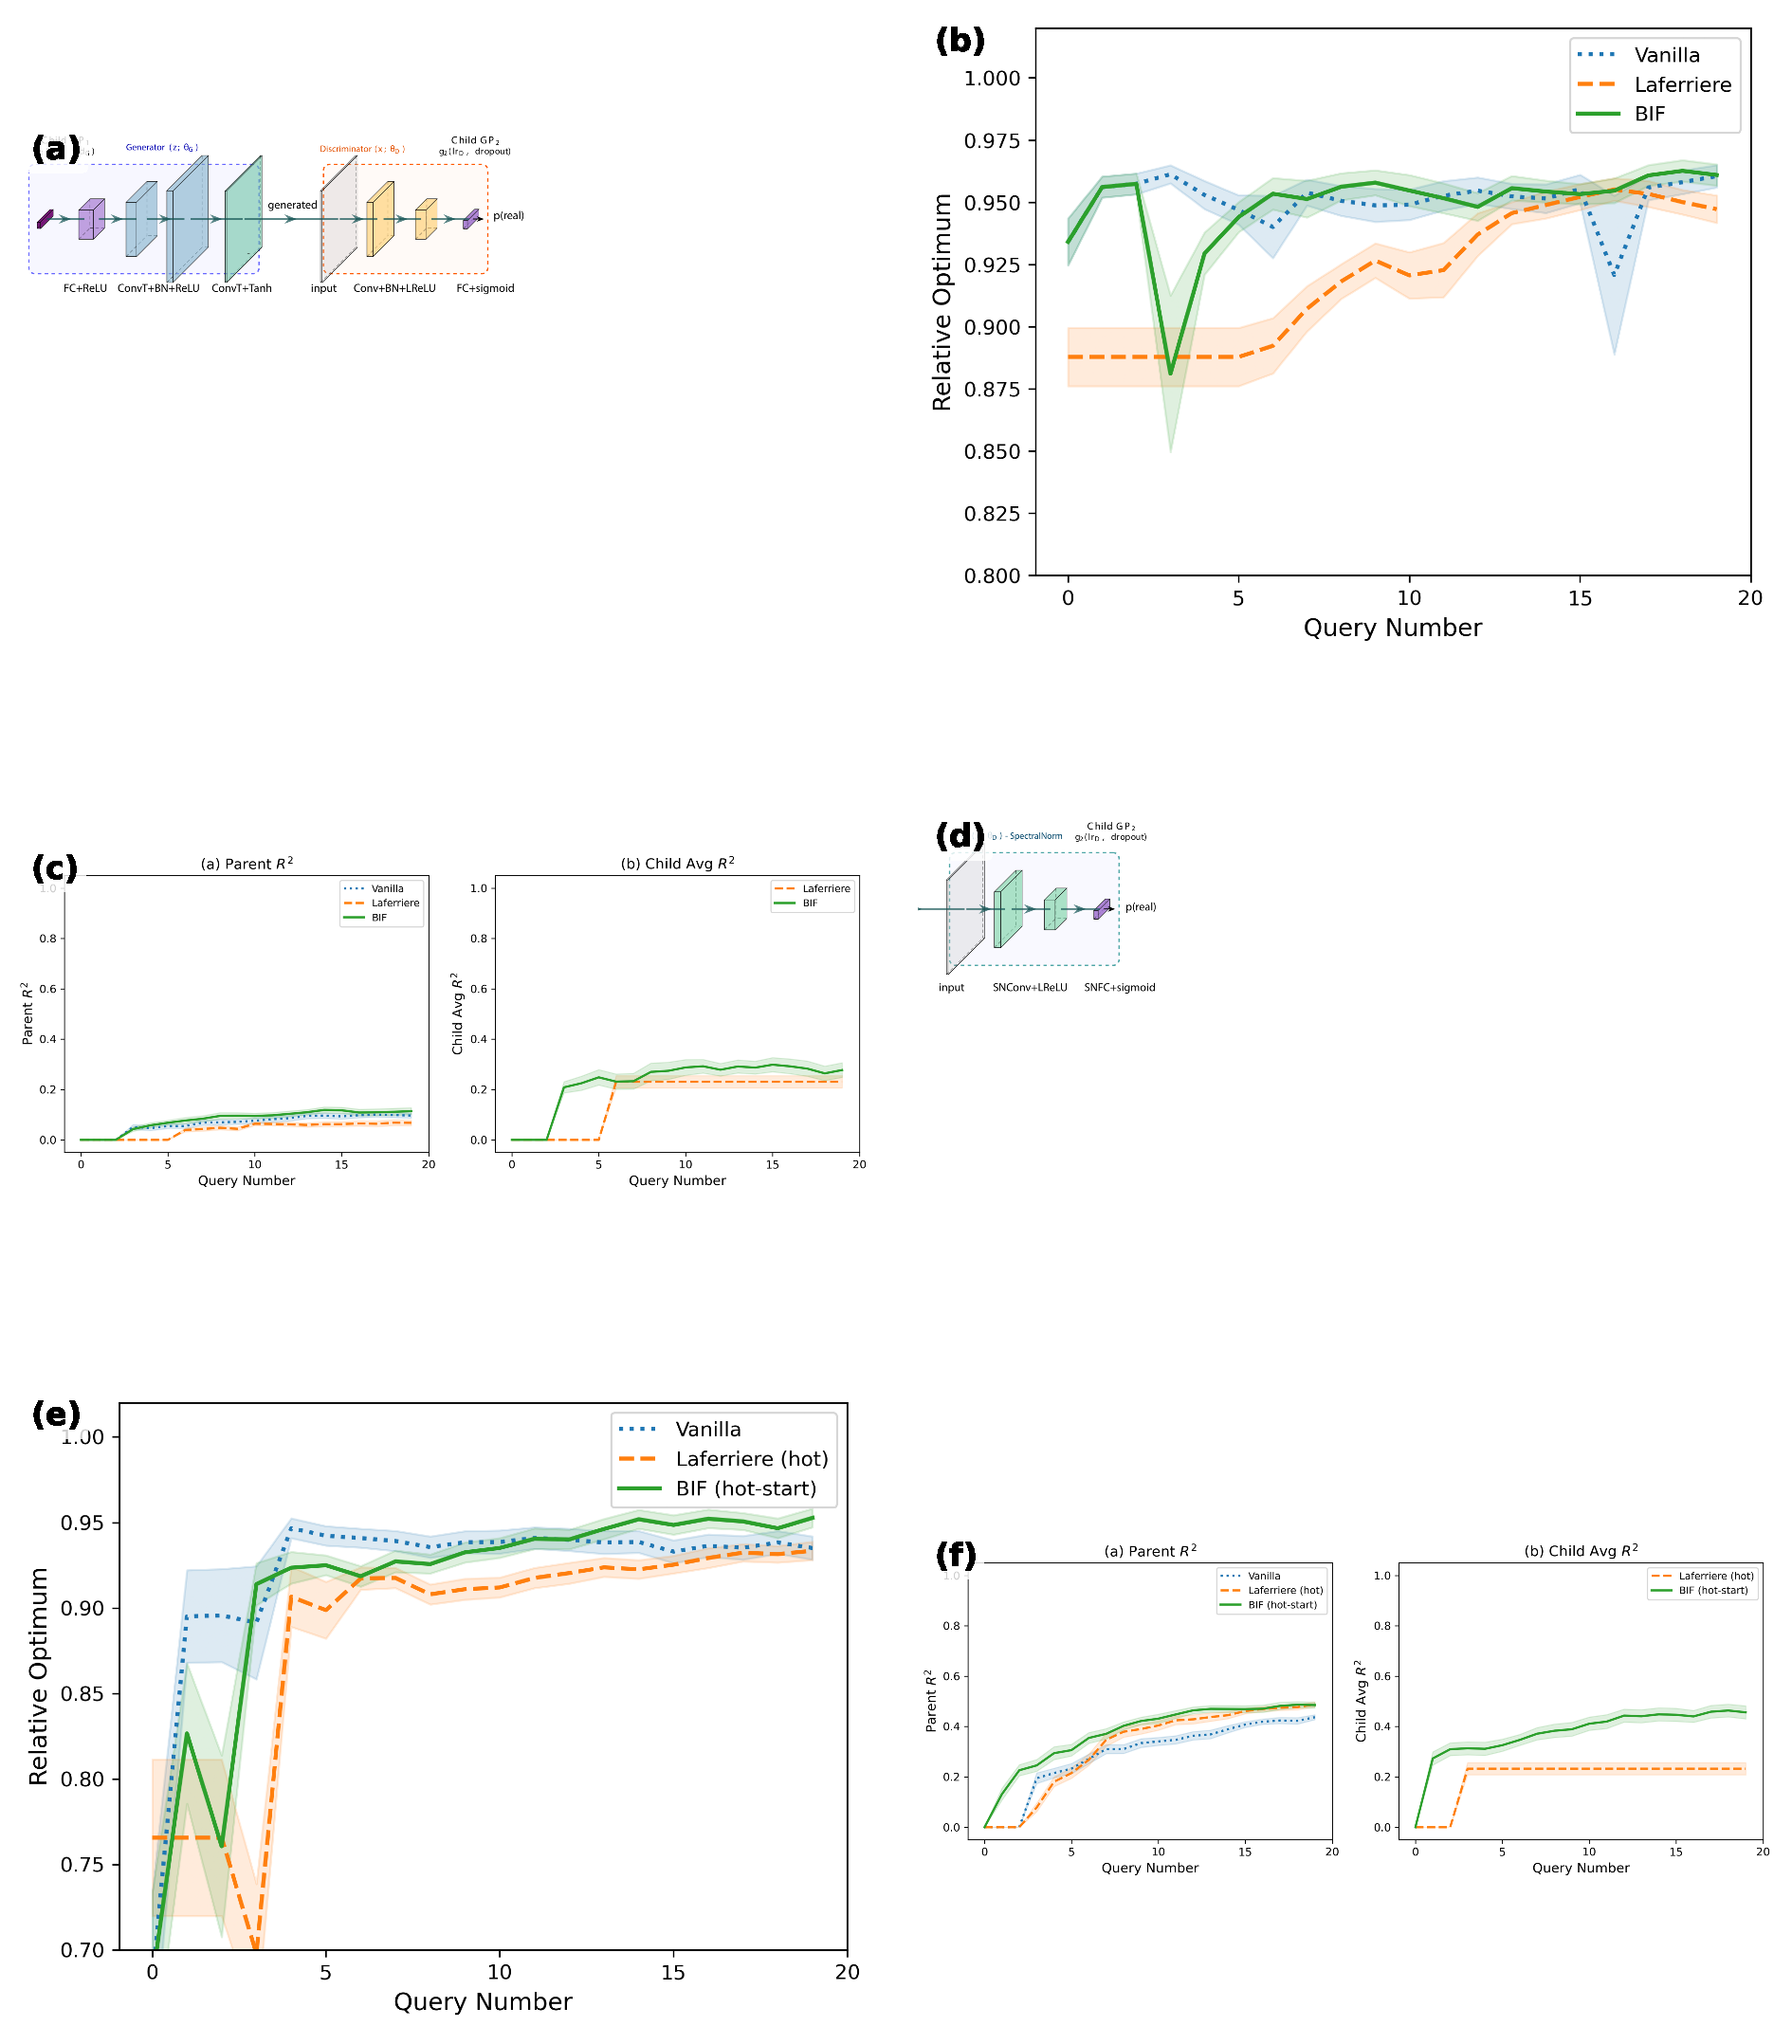
\includegraphics[width=\textwidth]{figures/figure4_composite.pdf}
\caption{GAN hyperparameter optimization experiment.
\textbf{(a)}~DCGAN architecture for the standard task
(generator: learning rate $\times$ weight decay;
discriminator: learning rate $\times$ dropout).
\textbf{(b)}~Relative Optimum on the standard task
(blue: Vanilla; orange: Laferri\`ere; green: BIF).
\textbf{(c)}~Parent and child $R^2$ on the standard task.
\textbf{(d)}~DCGAN architecture for the Spectral-Norm task
(shared generator, modified discriminator).
\textbf{(e)}~Relative Optimum on the modularity task
(Vanilla from scratch; Laferri\`ere and BIF hot-start with
transferred generator child).
\textbf{(f)}~Parent and child $R^2$ on the modularity task.
Shaded regions denote $\pm 1$ SEM over 30 seeds.}
\label{fig:gan}
\end{figure*}


% ============================================================================
% MODIFICATION 10: Abstract — UPDATE to mention GAN (optional, minor)
% Location: Abstract, the sentence listing evaluations.
% ============================================================================

\paragraph{Abstract --- update evaluation list (optional):}

% OLD: "...on synthetic and real-world neurostimulation optimization tasks."
% NEW:
...on synthetic, real-world neurostimulation, and realistic GAN hyperparameter
optimization tasks.


% ============================================================================
% SUMMARY OF ALL MODIFICATIONS
% ============================================================================
%
% 1.  Section 4 Datasets: change "three" -> "four", add GAN bullet
% 2.  Section 4 Implementation Details: add GAN hyperparams, update trial count
% 3.  Section 5 Results: add "GAN Hyperparameter Optimization" subsection
%     (after Neurostimulation, before Modularity)
% 4.  Section 5 Modularity: append GAN modularity paragraph
% 5.  Section 6 Conclusion: update empirical summary sentence
% 6.  Table 1: add 6 new rows (GAN HPO + GAN HPO Modularity)
% 7.  Figure 4: new composite figure (7 panels)
% 8.  Abstract: update evaluation list (optional)
%
% ============================================================================
\end{document}
